%
% Template for DCS course projects
%
\documentclass[a4paper,11pt,oneside]{book}
\usepackage[latin1]{inputenc}
\usepackage[english]{babel}
\usepackage{amsfonts}
\usepackage{amsmath}
\usepackage{amssymb,amsmath,color}
\usepackage{cite}
\usepackage{graphicx}
\usepackage{float}

\begin{document}
\pagestyle{myheadings}

%%%%%%%%%%% Cover %%%%%%%%%%%
\thispagestyle{empty}                                                 
\begin{center}                                                            
    \vspace{5mm}
    {\LARGE UNIVERSIT\`A DI BOLOGNA} \\                       
      \vspace{5mm}
\end{center}
\begin{center}
  
\includegraphics[scale=.27]{figs/logo_unibo}
\end{center}
\begin{center}
      \vspace{5mm}
      {\LARGE School of Engineering} \\
        \vspace{3mm}
      {\Large Master Degree in Automation Engineering} \\
      \vspace{20mm}
      {\LARGE Distributed Control Systems} \\
      \vspace{5mm}{\Large\textbf{COVERAGE CONTROL FOR COOPERATIVE MULTI-ROBOT NETWORKS}}                  
      \vspace{15mm}
\end{center}
\begin{flushleft}                                                                              
     {\large Professor: \textbf{\@ Giuseppe Notarstefano}} \\        
      \vspace{13mm}
\end{flushleft}
\begin{flushright}
      {\large Students:\\
      		\textbf{Donato Brusamento\\
      				Mattia Micozzi\\
      				Guido Carnevale\\
      				Lorenzo Draghetti}}\\
\end{flushright}        %capoverso allineato a destra
\begin{center}
\vfill
      {\large Academic year \@2018/2019} \\
\end{center}


\newpage
\thispagestyle{empty}

%%%%%% ABSTRACT %%%%%%%%%%


\begin{center}
\chapter*{}
\thispagestyle{empty}
{\Huge \textbf{Abstract}}\\
\vspace{15mm}
\end{center}
The aim of the project hereby presented was to transpose the algorithms described in the research paper\cite{K1} into a proper Matlab environment suitable for simulation and results analysis.\\\\

The aforementioned algorithms has been simplified in order to adapt to both an offline, sequential approach (from now on called \textbf{offline},or \textbf{centralized}) and to a parallel (single machine), asynchronous one (from now on called \textbf{online},or \textbf{distributed}).\\
In both approaches, the simulation implements a simple proportional closed loop control, but while in the former it is all done inside a centralized \textit{for loop}, in which informations about each agent is readily available to all others, in the latter we tried to be more faithful to the original formulation, in which every agents has to exchange with other agents informations about each other's positions in a timely manner, while being "deaf" (to a certain extent) in-between successive communications.\\\\

To achieve all of this we've made use of Matlab's \textit{Parallel Computing Toolbox} to simulate the independent agents as communicating threads.\\
In the distributed version of the simulation we also implemented a visual comparison between the two approaches so to show how they bring slightly different results.


%%%%%%%%%%%%%%%%%%%%%%%%%%%

\tableofcontents \thispagestyle{empty}
\listoffigures\thispagestyle{empty}

%%%%%% INTRODUZIONE %%%%%%%%%%
\chapter*{Introduction}
\addcontentsline{toc}{chapter}{Introduction}
A mobile wireless sensor network (MWSN) can be defined as a wireless sensor network (WSN) in which the sensor nodes are mobile. For example the nodes can be wheeled robots scattered in a given area.\\\\
MWSNs are an emerging field of research in contrast to their well-established predecessor. They are way more flexible than static sensor networks as they can be deployed in any scenario and deal with rapid topology changes due to node failures or new added sensors. In general each node consists of a radio transceiver, a microcontroller powered by a battery and one or more sensors to detect certain properties of the environment.~\cite{K2}\\ 
Typical applications of this kind of network are environment monitoring, surveillance, search and recovery operation, exploration.\\
A problem that can arise in this context is the optimization of coverage of a given area knowing the density distribution function, defined on that area, of a given property we would like to measure. The objective of this project was to implement a distributed and asynchronous algorithm to solve this problem, following the method proposed in the research paper \cite{K1}.\\\\
The considered framework, as suggested by the aforementioned paper, is the following: n mobile sensor-robots modelled as simple integrators strewn on an area given by a convex polytope defined in $\mathbb{R}^2$; on this area a 2-dimensional distribution $\phi:Q\rightarrow \mathbb{R}_+$ is defined to represent the density of the feature that nodes have to measure.\\ Each node has sensing (can locate the other nodes positions) and/or communication capabilities.  \\

Conceptually this algorithm runs iteratively 2 subroutines: one, called "Adjust-sensing radius algorithm", to compute the Voronoi cell of each sensor, and another one, called "Monitoring algorithm" to check if the computation of the Voronoi cell has to be updated because of significant changes in the network (variation of nodes positions, node failures,...).\\\\\\\\



We implemented this procedure in Matlab in 2 ways:
\begin{enumerate}
	\item in a centralized sequential way
	\item in a distributed parallel fashion, reading and writing files (stored in a master server) to realize communication among nodes.
\end{enumerate}
These two implementations and the differences between them are well-explained and analysed in this report\\
In particular, the first chapter regards the problem set-up and description of proposed solutions; the second chapter contains the analysis of obtained results.\\

 
\section*{Motivations}
The algorithms and simulations have been implemented in Matlab because of its (relatively speaking) simplicity and useful add-ons.\\
In particular, thanks to the graphical tools readily made available we could also create a real time results visualization to accompany the simulations, which is well suited to analyse the behaviour of both algorithm, compare them, and easily fix or add missing features.


\section*{Contributions}
We believe that, thanks to this project, we created a starting point for building and implementing on real MWSN the proposed control algorithms; while further steps have to be taken in the direction of optimizing the code for embedded platforms (and simulations as well), the main idea of the paper used as a guideline, and its efficiency, have been demonstrated through our framework.

%\section*{Organization}
%%%%%%%%%%%%%%%%%%%%%%%%%%%%%%%

%%%%%%%%% CAPITOLO  %%%%%%%%%%%%%%%%
\chapter{Chapter 1\\Problem set-up and solutions}
First-chapter for problem set-up and description of the implemented solution. 

\section{Setup}
\subsection {Theoretical notions}

The algorithm proposed by the main paper is \textbf{Lloyd's gradient descent}, which guarantees the convergence to an optimal solution intuitively given by the trade-off between each node's coverage (position) and relative degradation of sensing capabilities.\\
A main point to be considered is that this solution makes use of the concept of Voronoi partitions.\\\\

 Considering a convex polytope $Q$ in $\mathbb{R}^N$ and n sensors, for the sensor positions $P=\{p_1,...,p_n\}$ the optimal partition of $Q$ is the Voronoi partition  $V(P)=\{V_1,...,V_n\}$, where $V_i$ is the Voronoi cell of the i-th sensor: $$V_i=\{q\in Q|\> \|q-p_i\|\le\|q-p_j\|, \forall j\not= i\}$$\\
Intuitively speaking, each $V_i$ represents the region of space in which the respective sensor i is performing its task.\\

Citation \cite{K1}


\subsection{Adopted assumptions}

Although the code was implemented with the objective in mind of staying as much faithful to the paper as possible, some assumptions had to be made in order to work with the simulations running on a single machine, especially considering that some pieces of code (e.g. the computation of Voronoi cells) tend to slow them down quite a bit, and should then be optimized during further developments.\\ %(with a deeper proficiency of coding and mathematical skills that are unfortunately not in possession of anyone of us at the time of this writing).\\

In particular, with respect to the "ideal" version of the algorithm proposed in the paper\cite{K1}, the assumptions made are

\begin{enumerate}
	\item The \textit{sensing} of other agents is not implemented by a specific communication protocol; in the distribution version case, text files were written and read in a similar fashion to \textit{POSIX pipes}, and the only reason preventing an immediate sensing is the lock put to files during mutual r/w.\\This, as a side effects, also "forces" the lack of synchronism between threads.
	
	\item The \textit{timing}, as in the scheduling of different subroutines like monitoring and sensing, is not implemented, as it would require real platforms with only few unique threads running so to not introduce large discrepancies in convergence speeds.\\
	This is not only due to (rather severe) constraints of horsepower available on the used machines, but also to the lack of ready to use, POSIX-like scheduling primitives in Matlab's \textit{Parallel Computing Toolbox}.\\
	On top of that, while this would definitely be an issue in the real world implementation of the algorithm, for the purpose of this project (i.e. demonstration and simulation of the algorithm and creation of essential tools for its correct implementation), the proposed version suffices in its goals, and the following point explains the trade-off that was made in accordance with the professor's directions.
	
	\item For the same reason, while the correct calculation of neighbours weights is implemented and also displayed in the Offline algorithm, in the Distributed version agents do not wait for \textit{events} in order to change control, but rather they first reach the last computed region's centroid, and only then they sense others' position to update their own cell and reference centroid.\\
	However, should the need arise, the primitives and functions aiding in the event generation are already available in Ver. A of the code, as mentioned.
	
	
\end{enumerate}




\section{Inner Workings}
\subsection{Offline algorithm (A)}

As in Fig.~\ref{fig:algorithmA.png}... 

\begin{figure}
	
	\centering
	
	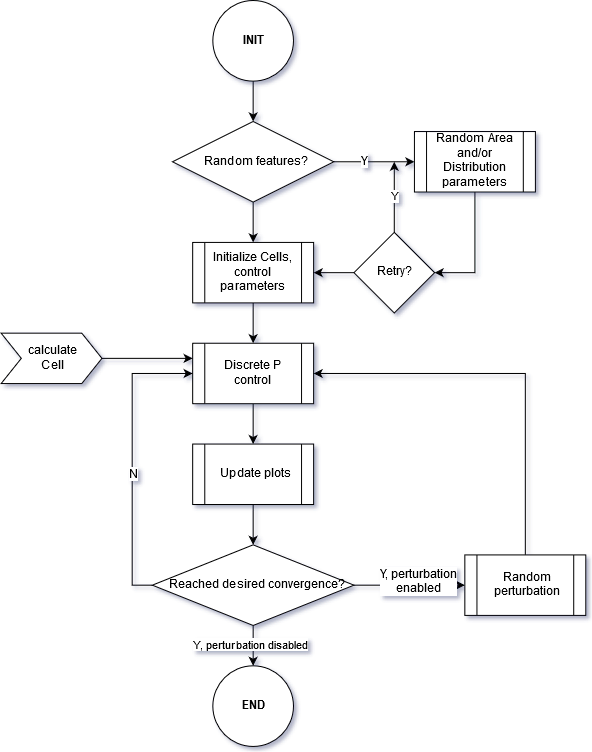
\includegraphics[scale=0.8]{figs/algorithmA.png}
	
	%%%%%%%%%%%%%%%%%%%%%%%%%%%%%%%%%%%%%%%%%inserisce la legenda ed etichetta
	%   la figura con \label{fig:prima}
	\caption{Algorithm A flow}\label{fig:algorithmA.png}
	
\end{figure}

\subsection{Online algorithm (B)}

\begin{figure}
	
	\centering
	
	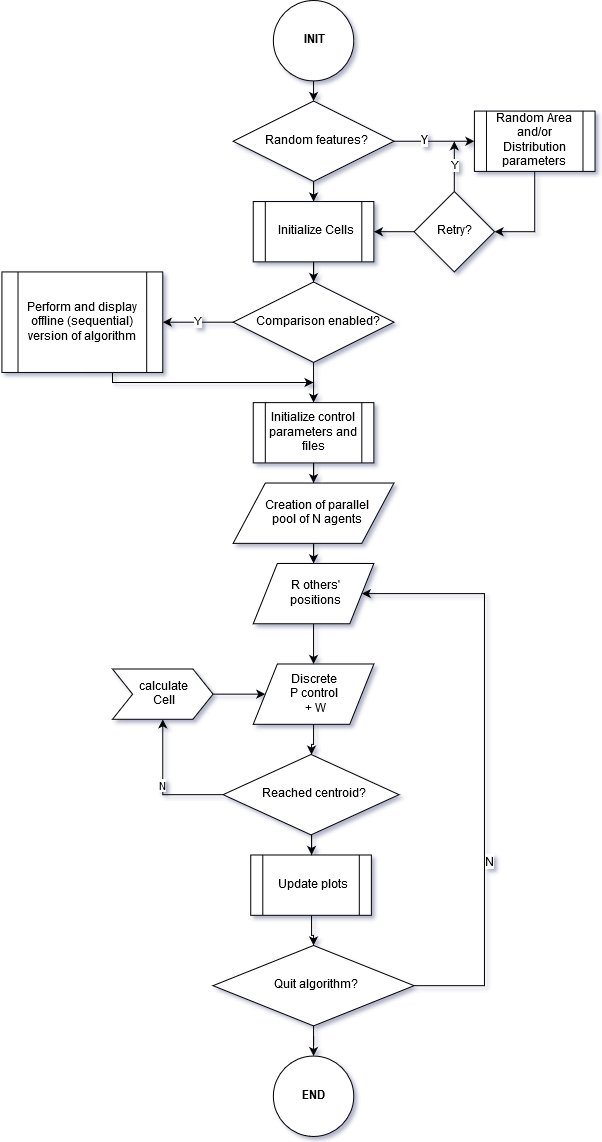
\includegraphics[scale=0.55]{figs/algorithmB.png}
	
	%%%%%%%%%%%%%%%%%%%%%%%%%%%%%%%%%%%%%%%%%inserisce la legenda ed etichetta
	%   la figura con \label{fig:prima}
	\caption{Algorithm B flow}\label{fig:algorithmB.png}
	
\end{figure}

\subsection{Utils}
\subsubsection{calculateCell}
\subsubsection{sliceCell}
\subsubsection{genMCGauss}


%%%%%%%%% CHAPTER  %%%%%%%%%%%%%%%%
\chapter{Chapter 2\\Results analysis}

\section{Prerequisites}
%put necessary toolboxes and FEX files here

Second chapter for description of the results (simulations and experiments where
applicable).
\section{Offline algorithm (A)}

%%%%%%%%%%%%%%%%%%%%%%%%%%%%%%%%%%%%%

%%%%% SVILUPPI FUTURI %%%%%%
\chapter*{Conclusions} % and future developments}
\addcontentsline{toc}{chapter}{Conclusions} %  and future developments}
%%%%%%%%%%%%%%%%%%%%%%%%%%

% %%%% APPENDIX %%%%%
% \appendix
% \chapter{Appendix title}
% %%%%%%%%%%%%%%%%%%%%

%%%%%%%%%% BIBLIOGRAPHY %%%%%%%%%%%%%%
\begin{thebibliography}{9}             %crea l'ambiente bibliografia

	%%%%%%%%%%%%%%%

\addcontentsline{toc}{chapter}{Bibliography}

\bibitem{K1} J. Cort�s, S. Mart�nez, T. Karatas, F. Bullo. "Coverage Control for Mobile Sensing Networks"
IEEE Transactions on Robotics and Automation, Vol. 20, No. 2, April 2004
\bibitem{K2} T. Hayes and F.H. Ali. "Mobile Wireless Sensor Networks: Applications and Routing Protocols" Handbook of Research on Next Generation Mobile Communications Systems. 2016.
%%%%%%%%%%%%%%%%%%%%%%%%%%%%%%%%%%%%%%

\end{thebibliography}


\end{document}
